\chapter{I/O structure}\label{}

%%%%%%%%%%%%%%%%%%%%%%%%%%%%%%%%%%%%%%%%%%%%%%%%%%%%%%%%%%%%%%%
\section{Output Options}
%%%%%%%%%%%%%%%%%%%%%%%%%%%%%%%%%%%%%%%%%%%%%%%%%%%%%%%%%%%%%%%
\begin{enumerate}
 \item \textbf{Dt output pixel}: is the delta time, expressed in hour, with which the
output for specified pixels is printed, [hour].\\
  \textsl{\small{parameters $\rightarrow$ control parameters $\rightarrow$ 6}}
 \item \textbf{Dt output basin}: is the delta time, expressed in hour, with which the
output for basin-altimetric rank values is printed (if applicable), [hour]\\
  \textsl{\small{parameters $\rightarrow$ control parameters $\rightarrow$ 7}}
 \item \textbf{ES num}: it represents how many altimetric stripes you want to
consider (up to 99); negative value means that this is done only for glacier
pixels, [-].\\
  \textsl{\small{parameters $\rightarrow$ control parameters $\rightarrow$ 8}}
 \item \textbf{format out}: is the output formats for the maps: 1 for
fluidturtle format, 2 for GRASS ASCII format, 3 for ESRI ASCII format, 4 for
NETCDF format, [-].\\
  \textsl{\small{parameters $\rightarrow$ control parameters $\rightarrow$ 11}}
 \item \textbf{Distr stat}: with the value 1 you choose to plot the 
  distribute statistics (min, max, var); whith 0 no statistic will be plotted, [-].\\
 \textsl{\small{parameters $\rightarrow$ options $\rightarrow$ base state parameters $\rightarrow$ 4}}
 \item \textbf{output Txy}: is the time interval (in hours) that you want the output 
  distibuited map to be plotted for the soil temperature, [hours].\\
 \textsl{\small{parameters $\rightarrow$ options $\rightarrow$ output parameters $\rightarrow$ 1}}
 \item \textbf{output TETAxy}: is the time interval (in hours) that you want the output 
  distibuited map to be plotted for the water content, [hours].\\
 \textsl{\small{parameters $\rightarrow$ options $\rightarrow$ output parameters $\rightarrow$ 2}}
 \item \textbf{output TETAICExy}: is the time interval (in hours) that you want the output 
  distibuited map to be plotted for the ice content, [hours].\\
 \textsl{\small{parameters $\rightarrow$ options $\rightarrow$ output parameters $\rightarrow$ 3}}
 \item \textbf{output PSIxy}: is the time interval (in hours) that you want the output 
  distibuited map to be plotted for the pore pressure, [hours].\\
 \textsl{\small{parameters $\rightarrow$ options $\rightarrow$ output parameters $\rightarrow$ 4}}
 \item \textbf{output snow}: is the time interval (in hours) that you want the output 
  distibuited map to be plotted for the snow thickness, [hours].\\
 \textsl{\small{parameters $\rightarrow$ options $\rightarrow$ output parameters $\rightarrow$ 5}}
 \item \textbf{output glac}: is the time interval (in hours) that you want the output 
  distibuited map to be plotted for the glacier thickness, [hours].\\
 \textsl{\small{parameters $\rightarrow$ options $\rightarrow$ output parameters $\rightarrow$ 6}}
 \item \textbf{output h sup}: is the time interval (in hours) that you want the output 
  distibuited map to be plotted for the height of the water table above the soil, [hours].\\
 \textsl{\small{parameters $\rightarrow$ options $\rightarrow$ output parameters $\rightarrow$ 7}}
 \item \textbf{output albedo}: is the time interval (in hours) that you want the output 
  distibuited map to be plotted for the albedo, [hours].\\
 \textsl{\small{parameters $\rightarrow$ options $\rightarrow$ output parameters $\rightarrow$ 8}}
 \item \textbf{output Rn}: is the time interval (in hours) that you want the output 
  distibuited map to be plotted for the Net Radiation, [hours]. \\
 \textsl{\small{parameters $\rightarrow$ options $\rightarrow$ output parameters $\rightarrow$ 9}}
 \item \textbf{output G}: is the time interval (in hours) that you want the output 
  distibuited map to be plotted for the Energy Flux, [hours].\\
 \textsl{\small{parameters $\rightarrow$ options $\rightarrow$ output parameters $\rightarrow$ 10}}
 \item \textbf{output H}: is the time interval (in hours) that you want the output 
  distibuited map to be plotted for the Sensible Heat Flux , [hours].\\
 \textsl{\small{parameters $\rightarrow$ options $\rightarrow$ output parameters $\rightarrow$ 11}}
 \item \textbf{output ET}: is the time interval (in hours) that you want the output 
  distibuited map to be plotted for the Evapo-Transpiration, [hours].\\
 \textsl{\small{parameters $\rightarrow$ options $\rightarrow$ output parameters $\rightarrow$ 12}}
 \item \textbf{output Ts}:type the time interval (in hours) that you want the output 
  distibuited map to be plotted for the Temperature at the surface, [hours].\\
 \textsl{\small{parameters $\rightarrow$ options $\rightarrow$ output parameters $\rightarrow$ 13}}
 \item \textbf{output P}: is the time interval (in hours) that you want the output 
  distibuited map to be plotted for the Precipitaion, [hours].\\
 \textsl{\small{parameters $\rightarrow$ options $\rightarrow$ output parameters $\rightarrow$ 14}}
 \item \textbf{output Wr}: is the time interval (in hours) that you want the output 
  distibuited map to be plotted for the Water Stored in the Vegetation, [hours].\\
 \textsl{\small{parameters $\rightarrow$ options $\rightarrow$ output parameters $\rightarrow$ 15}}
 \item \textbf{output SNOW}: is the time interval (in hours) that you want the output 
  distibuited map to be plotted for the snow melting and sublimation, [hours].\\
 \textsl{\small{parameters $\rightarrow$ options $\rightarrow$ output parameters $\rightarrow$ 16}}
 \item \textbf{output GLACIER}: is the time interval (in hours) that you want the output 
  distibuited map to be plotted for glacier melting and sublimation, [hours].\\
 \textsl{\small{parameters $\rightarrow$ options $\rightarrow$ output parameters $\rightarrow$ 17}}
 \item \textbf{output Rswdown}: is the time interval (in hours) that you want the output 
  distibuited map to be plotted for the Shortwave Radiation [hours].\\
 \textsl{\small{parameters $\rightarrow$ options $\rightarrow$ output parameters $\rightarrow$ 18}}
 \item \textbf{output meteo}: is the time interval (in hours) that you want the output
  distribuited map to be plotted for the meteo maps [hours].\\
 \textsl{\small{parameters $\rightarrow$ options $\rightarrow$ output parameters $\rightarrow$ 19}}
 \item \textbf{Special Output Parameters}: here is possible to select some days for which energy 
 balance and meteo data are plotted with a very short time step. This is useful if some careful analysis 
 has to be done. If you do not want to use this possibility, just write 0 as first
 component of this vector.\\
 \textsl{\small{parameters $\rightarrow$ options $\rightarrow$ special output $\rightarrow$ 1}}
\end{enumerate}

\begin{table}[!h]
\begin{footnotesize}
\begin{center}
\begin{tabular}{l|l|c|c|c}
&	name		&  unit 	  &  range of value 		 & default value \\
\hline
\#  1 &	Dt output pixel &	hour	& 	     .. 		&	0.5	\\
\#  2 &	Dt output basin	&	hour	&	     .. 		&	24	\\
\#  3 &	ES num		&	-	&	  -99 to 99 		&	1	\\
\#  4 &	format out	&	-	& 	    1 - 4 		&	2	\\
\#  5 &	distr stat	&	 -	&	0-1  			&	1	\\
\#  6 &	output Txy	&	 hr	& 0 - 1000 &	0	\\
\#  7 &	output TETAxy	& 	hr	& 0 - 1000 &	0.25	\\
\#  8 &	output TETAICExy& 	hr	& 0 - 1000 &	0	\\
\#  9 &	output PSIxy	& 	hr	& 0 - 1000 &	0.25	\\
\#  10 &	output snow	& 	hr	& 0 - 1000 &	0	\\
\#  11 &	output glac	& 	hr	& 0 - 1000 &	0	\\
\#  12 &	output h sup	& 	hr	& 0 - 1000 &	0	\\
\#  13 &	output albedo	& 	hr	& 0 - 1000 &	0	\\
\#  14 &	output Rn	& 	hr	& 0 - 1000 &	0	\\	
\#  15 &	output G	& 	hr	& 0 - 1000 &	0	\\	
\#  16 &	output H	& 	hr	& 0 - 1000 &	0	\\	
\#  17 &	output ET	& 	hr	& 0 - 1000 &	0	\\
\#  18 &	output Ts	& 	hr	& 0 - 1000 &	0	\\
\#  19 &	output P	& 	hr	& 0 - 1000 &	0	\\	
\#  20 &	output Wr	& 	hr	& 0 - 1000 &	0	\\
\#  21 &	output SNOW	& 	hr	& 0 - 1000 &	0	\\
\#  22 &	output GLACIER	& 	hr	& 0 - 1000 &	0	\\
\#  23 &	output Rswdown	& 	hr	& 0 - 1000 &	0	\\
\#  24 &	output meteo	& 	hr	& 0 - 1000 &	0	\\
\#  25 &Special Output Parameters & 	hr	&           &   0 	\\
\end{tabular}
\textsl{\caption{Output Options}\label{}}
 \end{center}
\end{footnotesize}
\end{table}



%%%%%%%%%%%%%%%%%%%%%%%%%%%%%%%%%%%%%%%%%%%%%%%%%%


\section{MONTEBELLO}


\begin{enumerate}
\item	\textbf{	DATE	}:		\\	$\rightarrow$	flows	$\rightarrow$	1
\item	\textbf{	JDfrom0	}:		\\	$\rightarrow$	flows	$\rightarrow$	2
\item	\textbf{	JD	}:		\\	$\rightarrow$	flows	$\rightarrow$	3
\item	\textbf{	Q\_tot	}	[$m^3 s^{-1}$]:	is the total discharge 	\\	$\rightarrow$	flows	$\rightarrow$	4
\item	\textbf{	Qsub\_ch	}	[$m^3 s^{-1}$]:	is the sub-superficial discharge	\\	$\rightarrow$	flows	$\rightarrow$	5
\item	\textbf{	Qsup\_ch	}	[$m^3 s^{-1}$]:	is the superficial discharge	\\	$\rightarrow$	flows	$\rightarrow$	6
\item	\textbf{	DATE	}:	is the date when the simulation oututps are plotted	\\	$\rightarrow$	basin	$\rightarrow$	1
\item	\textbf{	JDfrom0	}:	is the Julian Day when the simulation oututps are plotted	\\	$\rightarrow$	basin	$\rightarrow$	2
\item	\textbf{	JD	}:	is the Julian Day (with zero starting from the first of January of the year you are running the simulation) when the simulation oututps are plotted	\\	$\rightarrow$	basin	$\rightarrow$	3
\item	\textbf{	t\_i	}	[s]:	is the initial time, in seconds, of the interval when the outputs values are plotted	\\	$\rightarrow$	basin	$\rightarrow$	4
\item	\textbf{	t\_f	}	[s]:	is the final time, in seconds, of the interval when the outputs values are plotted	\\	$\rightarrow$	basin	$\rightarrow$	5
\item	\textbf{	Prain\_below\_canopy	}	[mm]:	is the rainfall precipitation which drops below the canopy	\\	$\rightarrow$	basin	$\rightarrow$	6
\item	\textbf{	Psnow\_below\_canopy	}	[mm]:	is the snow precipitation which drops below the canopy	\\	$\rightarrow$	basin	$\rightarrow$	7
\item	\textbf{	Prain\_above\_canopy	}	[mm]:	is the rainfall precipitation which falls above the canopy	\\	$\rightarrow$	basin	$\rightarrow$	8
\item	\textbf{	Psnow\_above\_canopy	}	[mm]:	is the snow precipitation which falls above the canopy	\\	$\rightarrow$	basin	$\rightarrow$	9
\item	\textbf{	Tair	}	[C]:	is the temperature of the air	\\	$\rightarrow$	basin	$\rightarrow$	10
\item	\textbf{	Tsurface	}	[C]:	is the temperature of the soil surface	\\	$\rightarrow$	basin	$\rightarrow$	11
\item	\textbf{	Tvegetation	}	[C]:	is the temperature of the vegetation	\\	$\rightarrow$	basin	$\rightarrow$	12
\item	\textbf{	Evap\_surface	}	[mm]:	is the evaporation from the surface	\\	$\rightarrow$	basin	$\rightarrow$	13
\item	\textbf{	Transpiration\_canopy	}	[mm]:	is the transpiration from the canopy	\\	$\rightarrow$	basin	$\rightarrow$	14
\item	\textbf{	LE	}	[$W m^{-2}$]:	is the latent heat flux at soil or snow surface	\\	$\rightarrow$	basin	$\rightarrow$	15
\item	\textbf{	H	}	[$W m^{-2}$]:	is the sensible heat flux at soil or snow surface	\\	$\rightarrow$	basin	$\rightarrow$	16
\item	\textbf{	SW	}	[$W m^{-2}$]:	is the short-wave raidiation at soil or snow surface	\\	$\rightarrow$	basin	$\rightarrow$	17
\item	\textbf{	LW	}	[$W m^{-2}$]:	is the long-wave emissivity at soil or snow surface	\\	$\rightarrow$	basin	$\rightarrow$	18
\item	\textbf{	LEv	}	[$W m^{-2}$]:	is the vegtation latent heat flux from leaves to canopy air	\\	$\rightarrow$	basin	$\rightarrow$	19
\item	\textbf{	Hv	}	[$W m^{-2}$]:	is the vegetation sensible heat flux from leaves to canopy air	\\	$\rightarrow$	basin	$\rightarrow$	20
\item	\textbf{	Swv	}	[$W m^{-2}$]:	is the vegetation short-wave raidiation adsobed by the vegetation	\\	$\rightarrow$	basin	$\rightarrow$	21
\item	\textbf{	Lwv	}	[$W m^{-2}$]:	is the vegetation long-wave radiation adsobed by the vegetation	\\	$\rightarrow$	basin	$\rightarrow$	22
\item	\textbf{	Swin	}	[$W m^{-2}$]:	is the incoming short-wave raidiation above vegetation	\\	$\rightarrow$	basin	$\rightarrow$	23
\item	\textbf{	Lwin	}	[$W m^{-2}$]:	is the incoming long-wave radiation above vegetation	\\	$\rightarrow$	basin	$\rightarrow$	24
\item	\textbf{	Mass\_balance\_error	}	[mm]:	is the error on the mass blance	\\	$\rightarrow$	basin	$\rightarrow$	25
\item	\textbf{	DATE	}:	is the date when the simulation oututps are plotted	\\		point	$\rightarrow$	1
\item	\textbf{	JDfrom0	}:	is the Julian Day when the simulation oututps are plotted	\\		point	$\rightarrow$	2
\item	\textbf{	JD	}:	is the Julian Day (with zero starting from the first of January of the year you are running the simulation) when the simulation oututps are plotted	\\		point	$\rightarrow$	3
\item	\textbf{	t	}	[d]:		\\		point	$\rightarrow$	4
\item	\textbf{	t\_i	}	[s]:	is the initial time, in seconds, of the interval when the outputs values are plotted	\\		point	$\rightarrow$	5
\item	\textbf{	t\_f	}	[s]:	is the final time, in seconds, of the interval when the outputs values are plotted	\\		point	$\rightarrow$	6
\item	\textbf{	Psnow\_over\_canopy	}	[mm]:	is the snow precipitation which falls over the canopy	\\		point	$\rightarrow$	7
\item	\textbf{	Prain\_over\_canopy	}	[mm]:	is the rainfall precipitation which falls above the canopy	\\		point	$\rightarrow$	8
\item	\textbf{	Psnow\_under\_canopy	}	[mm]:	is the snow precipitation which falls below the canopy	\\		point	$\rightarrow$	9
\item	\textbf{	Prain\_under\_canopy	}	[mm]:	is the rainfall precipitation which drops below the canopy	\\		point	$\rightarrow$	10
\item	\textbf{	Prain\_rain\_on\_snow	}	[mm]:	is the rainfall precipitation if falls when snow cover is present	\\		point	$\rightarrow$	11
\item	\textbf{	Wind speed	}	[$m s^{-1}$]:	is the wind speed	\\		point	$\rightarrow$	12
\item	\textbf{	Wind direction	}	[deg]:	is the wind direction	\\		point	$\rightarrow$	13
\item	\textbf{	Relative Humidity	}	[-]:	is the relative humidity	\\		point	$\rightarrow$	14
\item	\textbf{	Pressure	}	[kPa]:	is the atmospheric pressure	\\		point	$\rightarrow$	15
\item	\textbf{	Tair	}	[C]:	is the temperature of the air	\\		point	$\rightarrow$	16
\item	\textbf{	Tdew	}	[C]:	is the dew temperature of the air 	\\		point	$\rightarrow$	17
\item	\textbf{	Tsurface	}	[C]:	is the temperature of the soil surface	\\		point	$\rightarrow$	18
\item	\textbf{	Tvegetation	}	[C]:	is the temperature of the vegetation	\\		point	$\rightarrow$	19
\item	\textbf{	Tcanopyair	}	[C]:	is the temperature of the air inside the canopy	\\		point	$\rightarrow$	20
\item	\textbf{	Surface Energy balance	}	[$W m^{-2}$]:	is the net energy flux entering the soil or the snow	\\		point	$\rightarrow$	21
\item	\textbf{	Soil heat flux	}	[$W m^{-2}$]:	is the soil heat flux	\\		point	$\rightarrow$	22
\item	\textbf{	Swin	}	[$W m^{-2}$]:	is the incoming short-wave raidiation at soil or snow surface	\\		point	$\rightarrow$	23
\item	\textbf{	Swbeam	}	[$W m^{-2}$]:	is the direct short-wave radiation at soil or snow surface	\\		point	$\rightarrow$	24
\item	\textbf{	Swdiff	}	[$W m^{-2}$]:	is the diffuse short-wave radiation at soil or snow surface	\\		point	$\rightarrow$	25
\item	\textbf{	Lwin	}	[$W m^{-2}$]:	in the incoming long-wave radiation at soil or snow surface	\\		point	$\rightarrow$	26
\item	\textbf{	Lwin\_min	}	[$W m^{-2}$]:	in the minimum incoming long-wave radiation at soil or snow surface	\\		point	$\rightarrow$	27
\item	\textbf{	Lwin\_max	}	[$W m^{-2}$]:	in the maximum incoming long-wave radiation at soil or snow surface	\\		point	$\rightarrow$	28
\item	\textbf{	Swnet	}	[$W m^{-2}$]:	is the net short-wave radiation at soil or snow surface	\\		point	$\rightarrow$	29
\item	\textbf{	Lwnet	}	[$W m^{-2}$]:	is the net long-wave radiation at soil or snow surface	\\		point	$\rightarrow$	30
\item	\textbf{	H	}	[$W m^{-2}$]:	is the sensible heat flux at soil or snow surface	\\		point	$\rightarrow$	31
\item	\textbf{	LE	}	[$W m^{-2}$]:	is the latent heat flux at soil or snow surface	\\		point	$\rightarrow$	32
\item	\textbf{	Canopy fraction	}	[-]:	is the canopy fraction	\\		point	$\rightarrow$	33
\item	\textbf{	LAI	}	[$m^2 m^{-2}$]:	is the leaf area index	\\		point	$\rightarrow$	34
\item	\textbf{	z0veg	}	[m]:	is the surface roughness ?? in m?? negli input è in mm	\\		point	$\rightarrow$	35
\item	\textbf{	d0veg	}	[m]:	is the surface displacement heigth ?? in m?? negli input è in mm	\\		point	$\rightarrow$	36
\item	\textbf{	Estored\_canopy	}	[$W m^{-2}$]:	is the energy stored in the canopy	\\		point	$\rightarrow$	37
\item	\textbf{	Swv	}	[$W m^{-2}$]:	is the short-wave raidiation adsorbed by the vegetation	\\		point	$\rightarrow$	38
\item	\textbf{	Lwv	}	[$W m^{-2}$]:	in the long-wave radiation adsorbed by the vegetation	\\		point	$\rightarrow$	39
\item	\textbf{	Hv	}	[$W m^{-2}$]:	is the sensible heat flux from the vegetation from leaves to canopy air	\\		point	$\rightarrow$	40
\item	\textbf{	Lev	}	[$W m^{-2}$]:	is the latent heat flux from  the vegetation from leaves to canopy air	\\		point	$\rightarrow$	41
\item	\textbf{	Hg\_unveg	}	[$W m^{-2}$]:	is the sensible heat flux from the ground for the unvegetated areas from soil to atmosphere	\\		point	$\rightarrow$	42
\item	\textbf{	Leg\_unveg	}	[$W m^{-2}$]:	is the latent heat flux from the ground fot the vegetated areas from soil to atmosphere	\\		point	$\rightarrow$	43
\item	\textbf{	Hg\_veg	}	[$W m^{-2}$]:	is the sensible heat flux from the ground for the vegetated areas from soil to canopy air	\\		point	$\rightarrow$	44
\item	\textbf{	Leg\_veg	}	[$W m^{-2}$]:	is the latent heat flux from the ground for the vegetated areas from soil to canopy air	\\		point	$\rightarrow$	45
\item	\textbf{	Evap\_surface	}	[mm]:	is the evaporation from the surface	\\		point	$\rightarrow$	46
\item	\textbf{	Trasp\_canopy	}	[mm]:	is the transpiration from the canopy	\\		point	$\rightarrow$	47
\item	\textbf{	Water on canopy	}	[mm]:	is the water thickness on the canopy	\\		point	$\rightarrow$	48
\item	\textbf{	Snow on canopy	}	[mm]:	is the snow thickness on the canopy	\\		point	$\rightarrow$	49
\item	\textbf{	Qvegetation	}	[-]:	is the specific humidiy of the leaves surface ?	\\		point	$\rightarrow$	50
\item	\textbf{	Qsurface	}	[-]:	is the specific humidiy of the soil surface	\\		point	$\rightarrow$	51
\item	\textbf{	Qair	}	[-]:	is the specific humidiy of the  air	\\		point	$\rightarrow$	52
\item	\textbf{	Qcanopyair	}	[-]:	is the specific humidiy of the canopy air	\\		point	$\rightarrow$	53
\item	\textbf{	Lobukhov	}	[m]:	Monin - Obukhov length above the canopz	\\		point	$\rightarrow$	54
\item	\textbf{	Number of iter.	}:	of what?	\\		point	$\rightarrow$	55
\item	\textbf{	Lobukhovcanopy	}	[m]:	Monin - Obukhov length in the canopy	\\		point	$\rightarrow$	56
\item	\textbf{	Wind speed top canopy	}	[$m s^{-1}$]:	is the wind speed at the top of the canopy	\\		point	$\rightarrow$	57
\item	\textbf{	Decay of K in canopy	}	[-]:		\\		point	$\rightarrow$	58
\item	\textbf{	Swup	}	[$W m^{-2}$]:	is the short-wave raidiation emitted from both canopy and soil from soil and canopy to atmosphere	\\		point	$\rightarrow$	59
\item	\textbf{	Lwup	}	[$W m^{-2}$]:	is the long-wave radiation emitted from both canopy and soil from soil and canopy to atmosphere	\\		point	$\rightarrow$	60
\item	\textbf{	Hup	}	[$W m^{-2}$]:	is the sensible heat flux emitted from both canopy and soil from soil and canopy to atmosphere	\\		point	$\rightarrow$	61
\item	\textbf{	Leup	}	[$W m^{-2}$]:	is the latent heat flux emitted from both canopy and soil from soil and canopy to atmosphere	\\		point	$\rightarrow$	62
\item	\textbf{	snow melted	}	[mm]:	is the snow thickness that has been melted	\\		point	$\rightarrow$	63
\item	\textbf{	snow evap	}	[mm]:	is the snow thickness that has been evaporated	\\		point	$\rightarrow$	64
\item	\textbf{	snow subl	}	[mm]:	is the glacier thickness that has been sublimated	\\		point	$\rightarrow$	65
\item	\textbf{	glac melted	}	[mm]:	is the glacier thickness that has been melted	\\		point	$\rightarrow$	66
\item	\textbf{	glac evap	}	[mm]:	is the glacier thickness that has been evaporated	\\		point	$\rightarrow$	67
\item	\textbf{	glac subl	}	[mm]:	is the glacier thickness that has been sublimated	\\		point	$\rightarrow$	68
\item	\textbf{	DATE	}:	is the date when the simulation oututps are plotted	\\		snow	$\rightarrow$	1
\item	\textbf{	JDfrom0	}:	is the Julian Day when the simulation oututps are plotted	\\		snow	$\rightarrow$	2
\item	\textbf{	JD	}:	is the Julian Day (with zero starting from the first of January of the year you are running the simulation) when the simulation oututps are plotted	\\		snow	$\rightarrow$	3
\item	\textbf{	t\_i[s]	}	[s]:	is the initial time, in seconds, of the interval when the outputs values are plotted	\\		snow	$\rightarrow$	4
\item	\textbf{	t\_f[s]	}	[s]:	is the final time, in seconds, of the interval when the outputs values are plotted	\\		snow	$\rightarrow$	5
\item	\textbf{	Snowtype	}	[-]:	is the type of snow	\\		snow	$\rightarrow$	6
\item	\textbf{	Snowdepth	}	[mm]:	is the depth of the snow	\\		snow	$\rightarrow$	7
\item	\textbf{	SWE	}	[mm]:	is the snow water equivalent	\\		snow	$\rightarrow$	8
\item	\textbf{	Temp\_aver	}	[C]:	is the avrage temperature	\\		snow	$\rightarrow$	9
\item	\textbf{	Density\_aver	}	[$kg m^{-3}$]:	is the average density of the snow	\\		snow	$\rightarrow$	10
\item	\textbf{	melting	}	[mm]:	is the snow that has been melted	\\		snow	$\rightarrow$	11
\item	\textbf{	sublimation	}	[mm]:	is the snow that has been sublimated	\\		snow	$\rightarrow$	12
\item	\textbf{	evaporation	}	[mm]:	is the snow that has been evaporated	\\		snow	$\rightarrow$	13
\item	\textbf{	nlayer	}	[-]:	is the number of layer of snow which have been created during the simulation	\\		snow	$\rightarrow$	14
\item	\textbf{	Bstrans	}	[mm]:	is the blowing snow �??? trans???	\\		snow	$\rightarrow$	15
\item	\textbf{	Bstrans\_cum	}	[mm]:		\\		snow	$\rightarrow$	16
\item	\textbf{	Bssubl	}	[mm]:		\\		snow	$\rightarrow$	17
\item	\textbf{	Bssubl\_cum	}	[mm]:		\\		snow	$\rightarrow$	18
\item	\textbf{	Bstot	}	[mm]:	is the total blowing snow	\\		snow	$\rightarrow$	19
\item	\textbf{	Bstot\_cum	}	[mm]:		\\		snow	$\rightarrow$	20
\item	\textbf{	Dlayer\_1	}	[mm]:	is the thickness of the first layer of snow	\\		snow	$\rightarrow$	21
\item	\textbf{	Dlayer\_2	}	[mm]:	is the thickness of the second layer of snow	\\		snow	$\rightarrow$	22
\item	\textbf{	Dlayer\_3	}	[mm]:	is the thickness of the third layer of snow	\\		snow	$\rightarrow$	23
\item	\textbf{	Dlayer\_4	}	[mm]:	is the thickness of the fourth layer of snow	\\		snow	$\rightarrow$	24
\item	\textbf{	Dlayer\_5	}	[mm]:	is the thickness of the fifth layer of snow	\\		snow	$\rightarrow$	25
\item	\textbf{	Zlayer\_1	}	[mm]:	is the height of the first layer of snow	\\		snow	$\rightarrow$	26
\item	\textbf{	Zlayer\_2	}	[mm]:	is the height of the second layer of snow	\\		snow	$\rightarrow$	27
\item	\textbf{	Zlayer\_3	}	[mm]:	is the height of the third layer of snow	\\		snow	$\rightarrow$	28
\item	\textbf{	Zlayer\_4	}	[mm]:	is the height of the fourth layer of snow	\\		snow	$\rightarrow$	29
\item	\textbf{	Zlayer\_5	}	[mm]:	is the height of the fifth layer of snow	\\		snow	$\rightarrow$	30
\item	\textbf{	Temp\_1	}	[C]:	is the temperaure of the snow at the first layer	\\		snow	$\rightarrow$	31
\item	\textbf{	Temp\_2	}	[C]:	is the temperaure of the snow at the second layer	\\		snow	$\rightarrow$	32
\item	\textbf{	Temp\_3	}	[C]:	is the temperaure of the snow at the third layer	\\		snow	$\rightarrow$	33
\item	\textbf{	Temp\_4	}	[C]:	is the temperaure of the snow at the fourth layer	\\		snow	$\rightarrow$	34
\item	\textbf{	Temp\_5	}	[C]:	is the temperaure of the snow at the fifth layer	\\		snow	$\rightarrow$	35
\item	\textbf{	Density\_1	}	[$kg m^{-3}$]:	is the density of the first layer of snow	\\		snow	$\rightarrow$	36
\item	\textbf{	Density\_2	}	[$kg m^{-3}$]:	is the density of the second layer of snow	\\		snow	$\rightarrow$	37
\item	\textbf{	Density\_3	}	[$kg m^{-3}$]:	is the density of the third layer of snow	\\		snow	$\rightarrow$	38
\item	\textbf{	Density\_4	}	[$kg m^{-3}$]:	is the density of the fourth layer of snow	\\		snow	$\rightarrow$	39
\item	\textbf{	Density\_5	}	[$kg m^{-3}$]:	is the density of the fifth layer of snow	\\		snow	$\rightarrow$	40
\item	\textbf{	SWE\_1	}	[mm]:	is the snow water equivalent of the first layer of snow	\\		snow	$\rightarrow$	41
\item	\textbf{	SWE\_2	}	[mm]:	is the snow water equivalent of the second layer of snow	\\		snow	$\rightarrow$	42
\item	\textbf{	SWE\_3	}	[mm]:	is the snow water equivalent of the third layer of snow	\\		snow	$\rightarrow$	43
\item	\textbf{	SWE\_4	}	[mm]:	is the snow water equivalent of the fourth layer of snow	\\		snow	$\rightarrow$	44
\item	\textbf{	SWE\_5	}	[mm]:	is the snow water equivalent of the fifth layer of snow	\\		snow	$\rightarrow$	45
\item	\textbf{	ice\_1	}	[$kg m^{-2}$]:	is the ice quantity on the first layer of snow	\\		snow	$\rightarrow$	46
\item	\textbf{	ice\_2	}	[$kg m^{-2}$]:	is the ice quantity of the second layer of snow	\\		snow	$\rightarrow$	47
\item	\textbf{	ice\_3	}	[$kg m^{-2}$]:	is the ice quantity of the third layer of snow	\\		snow	$\rightarrow$	48
\item	\textbf{	ice\_4	}	[$kg m^{-2}$]:	is the ice quantity of the fourth layer of snow	\\		snow	$\rightarrow$	49
\item	\textbf{	ice\_5	}	[$kg m^{-2}$]:	is the ice quantity of the fifth layer of snow	\\		snow	$\rightarrow$	50
\item	\textbf{	water\_1	}	[$kg m^{-2}$]:	is the water quantity on the first layer of snow	\\		snow	$\rightarrow$	51
\item	\textbf{	water\_2	}	[$kg m^{-2}$]:	is the water quantity of the second layer of snow	\\		snow	$\rightarrow$	52
\item	\textbf{	water\_3	}	[$kg m^{-2}$]:	is the water quantity of the third layer of snow	\\		snow	$\rightarrow$	53
\item	\textbf{	water\_4	}	[$kg m^{-2}$]:	is the water quantity of the fourth layer of snow	\\		snow	$\rightarrow$	54
\item	\textbf{	water\_5	}	[$kg m^{-2}$]:	is the water quantity of the fifth layer of snow	\\		snow	$\rightarrow$	55
\end{enumerate}


%%%%%%%%%%%%%%%%%%%%%%%%%%%%%%%%%%%%%%%%%%%%%%%%%%%%%%%%%%%%%%%%
\section{Tabs}
%%%%%%%%%%%%%%%%%%%%%%%%%%%%%%%%%%%%%%%%%%%%%%%%%%%%%%%%%%%%%%%%

%%=============================================================%
\subsection{Flows}
%%=============================================================%
It gives the value of the total, the sub-superficial and superficial discharge in:
\begin{itemize}
 \item point simulation: the point of interest 
 \item distributed simulation: the closure section of the basin
\end{itemize}

\begin{figure}[!htbp]
\begin{center}
  \begin{minipage}[c]{0.5\textwidth}
  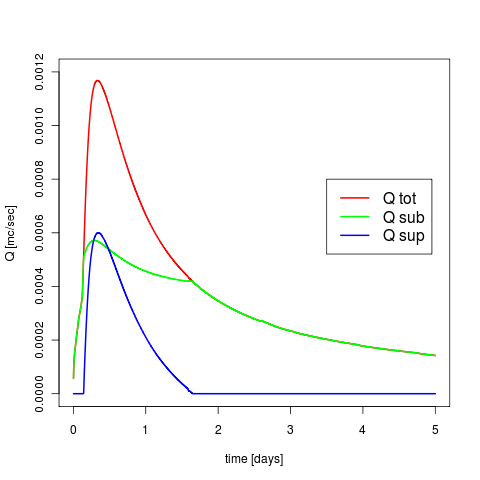
\includegraphics[width=1.0\textwidth]{./images/Q_200.png}
  \end{minipage}
\end{center}
\textsl{\caption{Plot (obtained with R) of the discharge dat in the closure section}\label{}}
\end{figure}

Below is the header of the oputput file.
\begin{table}[!h]
\begin{footnotesize}
\begin{center}
\begin{tabular}{c|c|c|c|c|c|c}
DATE	& JDfrom0  &	JD     &    Q\_tot	   &  Qsub\_ch	&  Qsup\_ch      &	Q\_G \\
\hline
[-]	&      [-]  &	[-]   &    [mc/s]        &  [mc/s]	&  [mc/s]        &	[mc/s] \\

\end{tabular}
\textsl{\caption{Flow}\label{}}
 \end{center}
\end{footnotesize}
\end{table}




%%=============================================================%
\subsection{Basin}
%%=============================================================%
This file contains 50 parameters which are averaged in the whole basin.
\begin{enumerate}
  \item \textbf{DATE}: is the date when	the simulation oututps are plotted;
  \item \textbf{JDfrom0}: is the Julian Day when the simulation oututps are plotted;	
  \item \textbf{JD}: is the Julian Day (with zero starting from the first of January 
  of the yoear you are running the simulation) when the simulation oututps are plotted;	
  \item \textbf{t\_i} [s]: is the initial time, in seconds, of the interval when the outputs values are plotted;	
  \item \textbf{t\_f} [s]: is the final time, in seconds, of the interval when the outputs values are plotted;
  \item \textbf{Esoil} \textcolor{red}{?????} [mm]
  \item \textbf{Ecv} \textcolor{red}{?????} [mm]
  \item \textbf{Etc} \textcolor{red}{?????} [mm]
  \item \textbf{SW}: is the short-wave raidiation [$W/m^2$]
  \item \textbf{LW}: is the long-wave radiation [$W/m^2$]
  \item \textbf{H}: is the sensible heat flux [$W/m^2$]
  \item \textbf{LE}: is the latent heat of evaporation [$W/m^2$]
  \item \textbf{SWv}: is the short-wave raidiation of the vegetation [$W/m^2$]
  \item \textbf{LWv}: is the long-wave radiation of the vegetation [$W/m^2$]
  \item \textbf{Hv}: is the sensible heat flux of the vegetation [$W/m^2$]
  \item \textbf{LEv}: is the latent heat of evaporation of the vegetation[$W/m^2$]
  \item \textbf{Ta}: is the temperature of the air [\textdegree C] \textcolor{red}{?????}
  \item \textbf{Tg}: is the temperature of the ..... [\textdegree C]
  \item \textbf{Tv}: is the temperature of the vegetation [\textdegree C] \textcolor{red}{?????}
  \item \textbf{SWin}: is the incoming short-wave raidiation [\textdegree C]
  \item \textbf{Prain}: is the rainfall precipitation [mm] \textcolor{red}{?????}
  \item \textbf{Psnow}: is the snow precipitation [mm] \textcolor{red}{?????} 
  \item \textbf{Dwt} [mm] \textcolor{red}{?????} 
  \item \textbf{Pn}: is the net precipitation [mm] \textcolor{red}{?????} 
  \item \textbf{Infiltration}: is the infiltration into the soil [mm] \textcolor{red}{?????} 
  \item \textbf{DS\_sup}: is the diffuse radiation coming from the sky [mm] \textcolor{red}{?????}  
  \item \textbf{DS\_sub}:  is the diffuse radiation coming from the sky  [mm] \textcolor{red}{?????} 
  \item \textbf{DS\_ch}:  is the diffuse radiation coming from the sky  [mm] \textcolor{red}{?????} 
  \item \textbf{R\_G} [mm] \textcolor{red}{?????} 
  \item \textbf{R\_tot} [mm] \textcolor{red}{?????} 
  \item \textbf{SSup} [mm] \textcolor{red}{?????} 
  \item \textbf{SSub} [mm] \textcolor{red}{?????} 
  \item \textbf{wt} [mm] \textcolor{red}{?????} 
  \item \textbf{SWE} [mm] \textcolor{red}{?????} 
  \item \textbf{D\_SWE} [mm] \textcolor{red}{?????} 
  \item \textbf{MeltSnow} [mm] \textcolor{red}{?????} 
  \item \textbf{D\_MeltSnow} [mm] \textcolor{red}{?????} 
  \item \textbf{SublSnow} [mm] \textcolor{red}{?????} 
  \item \textbf{D\_SublSnow} [mm] \textcolor{red}{?????} 	
  \item \textbf{EvapSnow} [mm] \textcolor{red}{?????} 	
  \item \textbf{D\_EvapSnow} [mm] \textcolor{red}{?????} 	
  \item \textbf{GWE} [mm] \textcolor{red}{?????} 
  \item \textbf{D\_GWE} [mm] \textcolor{red}{?????} 	
  \item \textbf{MeltGlac} [mm] \textcolor{red}{?????} 	
  \item \textbf{D\_MeltGlac} [mm]	\textcolor{red}{?????} 
  \item \textbf{SublGlac} [mm]	\textcolor{red}{?????} 
  \item \textbf{D\_SublGlac} [mm]	\textcolor{red}{?????} 
  \item \textbf{EvapGlac} [mm]	\textcolor{red}{?????} 
  \item \textbf{D\_EvapGlac} [mm]	\textcolor{red}{?????} 
  \item \textbf{ErrorRichards} [mm $h^{-1}$] \textcolor{red}{?????} 
\end{enumerate}

%%=============================================================%
\subsection{Point}
%%=============================================================%
All the following proprieties are calculated in the specified check point.
In a distributed simulation for every check point will be created a file 
with the following proprieties (in point simulation is possible to specify just one point, so only one
file will be created).


\begin{enumerate}
  \item \textbf{DATE}: is the date when	the simulation outputs are plotted;
  \item \textbf{JDfrom0}: is the Julian Day when the simulation outputs are plotted;	
  \item \textbf{JD}: is the Julian Day (with zero starting from the first of January 
  of the yoear you are running the simulation) when the simulation outputs are plotted;	
  \item \textbf{t} [decimal]: is the decimal time when the simulation outputs 
  \item \textbf{t\_i} [s]: is the initial time, in seconds, of the interval when the outputs values are plotted;	
  \item \textbf{t\_f} [s]: is the final time, in seconds, of the interval when the outputs values are plotted;
  \item \textbf{v} [m/s]: is the water velocity in the check point \textcolor{red}{?????} 
  \item \textbf{Vdir}: is the direction of ......	\textcolor{red}{?????} 
  \item \textbf{RH}: is the rlative humidity [-]	\textcolor{red}{?????} 
  \item \textbf{P}: is the air pressure [hPa]	\textcolor{red}{?????} 
  \item \textbf{Tair}: is the temperature of the air [C]	\textcolor{red}{?????} 
  \item \textbf{Tsurface}: is the temperature of the surface [C]	\textcolor{red}{?????} 
  \item \textbf{Tdew}: is the temperature of the dew [C]	\textcolor{red}{?????} 
  \item \textbf{eair}  [mbar]	\textcolor{red}{?????} 
  \item \textbf{Qair}: is the energy flux due to soil-atmosphere iteractions [-]	\textcolor{red}{?????} 
  \item \textbf{esurf} [mbar]	\textcolor{red}{?????} 
  \item \textbf{Qsurf}: is the energy flux due to soil-atmosphere iteractions [-]	\textcolor{red}{?????} 
  \item \textbf{SWin}: is the short wave radiation [W$m^{-2}$]	\textcolor{red}{?????} 
  \item \textbf{SWin\_beam}: is the short wave radiation 	\textcolor{red}{?????} 
  \item \textbf{SWin\_diff}: is the short wave radiation 	\textcolor{red}{?????} 
  \item \textbf{SWout}: is the short wave [W$m^{-2}$]	\textcolor{red}{?????} 
  \item \textbf{alpha} [deg]	\textcolor{red}{?????} 
  \item \textbf{direction} [deg]	\textcolor{red}{?????} 
  \item \textbf{phi} [deg]	\textcolor{red}{?????} 
  \item \textbf{LWin}: is the long wave radiation  [W$m^{-2}$]	\textcolor{red}{?????} 
  \item \textbf{LWout}: is the long wave radiation  [W$m^{-2}$]	\textcolor{red}{?????} 
  \item \textbf{Rnet}: is the net radiation [W$m^{-2}$] \textcolor{red}{?????} 
  \item \textbf{SW}: is the short wave radiation  [W$m^{-2}$]	\textcolor{red}{?????} 
  \item \textbf{LW}: is the long wave radiation  [W$m^{-2}$]	\textcolor{red}{?????} 
  \item \textbf{H}: is the sensible heat flux [W$m^{-2}$]	\textcolor{red}{?????} 
  \item \textbf{LE}: is the latent heat of evaporation [W$m^{-2}$]	\textcolor{red}{?????} 
  \item \textbf{Qrain}: is the energy flux due to soil-atmosphere iteractions  [W$m^{-2}$]	\textcolor{red}{?????} 
  \item \textbf{Gsoil}: is the energy flux in the soil per unit area due to heat conduction [W$m^{-2}$]	\textcolor{red}{?????} 
  \item \textbf{SurfaceEB} [W$m^{-2}$]	\textcolor{red}{?????} 
  \item \textbf{SWin\_c}: is the short wave radiation [MJ]	\textcolor{red}{?????} 
  \item \textbf{SWout\_c}: is the short wave radiation [MJ]	\textcolor{red}{?????} 
  \item \textbf{LWin\_c}: is the long wave radiation [MJ]	\textcolor{red}{?????} 
  \item \textbf{LWout\_c}: is the long wave radiation [MJ]	\textcolor{red}{?????} 
  \item \textbf{SW\_cum}: is the shot wave radiation [MJ]	\textcolor{red}{?????} 
  \item \textbf{LWn\_cum}: is the long wave radiation [MJ]	\textcolor{red}{?????} 
  \item \textbf{Rnet\_cm}: is the net radiation [MJ]	\textcolor{red}{?????} 
  \item \textbf{H\_cum}: is the sensible heat flux [MJ]	\textcolor{red}{?????} 
  \item \textbf{LE\_cum}: is the latent heat of evaporation [MJ]	\textcolor{red}{?????} 
  \item \textbf{G\_cum}: is the energy flux in the soil per unit area due to heat conduction [MJ]	\textcolor{red}{?????} 
  \item \textbf{Eg} [mm]	\textcolor{red}{?????} 
  \item \textbf{Sg} [mm]	\textcolor{red}{?????} 
  \item \textbf{Etc} [mm]	\textcolor{red}{?????} 
  \item \textbf{Psnow}: is the snow precipitation [mm]	\textcolor{red}{?????} 
  \item \textbf{Prain}: is the rain precipitation [mm]	\textcolor{red}{?????} 
  \item \textbf{Psnow\_c}: is the snow precipitation [mm]	\textcolor{red}{?????} 
  \item \textbf{Prain\_SOILc}: is the rain precipitation  [mm]	\textcolor{red}{?????} 
  \item \textbf{Prain\_SNOWc}: is the rain precipitation  [mm]	\textcolor{red}{?????} 
  \item \textbf{Ptot\_c}: is the total rain precipitation [mm]	\textcolor{red}{?????} 
  \item \textbf{Wtrain} [mm]	\textcolor{red}{?????} 
  \item \textbf{Wtsnow} [mm]	\textcolor{red}{?????} 
  \item \textbf{Ptot\_atm}:  	\textcolor{red}{?????} 
  \item \textbf{Rain\_atm}	\textcolor{red}{?????} 
  \item \textbf{Snow\_atm}	\textcolor{red}{?????} 
  \item \textbf{Ptot\_atm\_cum}	 \textcolor{red}{?????} 
  \item \textbf{Prain\_atm\_cum}	\textcolor{red}{?????} 
  \item \textbf{Psnow\_atm\_cum}	\textcolor{red}{?????} 
  \item \textbf{Pn} [mm]	\textcolor{red}{?????} 
  \item \textbf{Runoff} [mm]	\textcolor{red}{?????} 
  \item \textbf{q\_sup}: is the superficial discharge [mm]	\textcolor{red}{?????} 
  \item \textbf{q\_sub}: is the sub-superficial discharge [mm]	\textcolor{red}{?????} 
  \item \textbf{DS\_sup} [mm]	\textcolor{red}{?????} 
  \item \textbf{DS\_sub} [mm]	\textcolor{red}{?????} 
  \item \textbf{q\_G} [mm]	\textcolor{red}{?????} 
  \item \textbf{snowDEPTH} [mm]	\textcolor{red}{?????} 
  \item \textbf{SWE} [mm]	\textcolor{red}{?????} 
  \item \textbf{snowDENSITY}: is the snow desity [$kg$ $m^{-3}$]	\textcolor{red}{?????} 
  \item \textbf{snowT}: is the snow temperature [C]	\textcolor{red}{?????} 
  \item \textbf{BStot} [mm]	\textcolor{red}{?????} 
  \item \textbf{BStot\_cum} [mm]	\textcolor{red}{?????} 
  \item \textbf{snowMELT} [mm]	\textcolor{red}{?????} 
  \item \textbf{snowSUBL} [mm]	\textcolor{red}{?????} 
  \item \textbf{snowEVAP} [mm]	\textcolor{red}{?????} 
  \item \textbf{glacierDEPTH} [mm]	\textcolor{red}{?????} 
  \item \textbf{GWE} [mm]	\textcolor{red}{?????} 
  \item \textbf{gDENSITY} [$kg$ $m^{-3}$]	\textcolor{red}{?????} 
  \item \textbf{glcT} [C]	\textcolor{red}{?????} 
  \item \textbf{glcMELT} [mm]	\textcolor{red}{?????} 
  \item \textbf{glcSUBL} [mm]	\textcolor{red}{?????} 
  \item \textbf{glcEVAP} [mm]	\textcolor{red}{?????} 
  \item \textbf{qv} [mm/d]	\textcolor{red}{?????} 
  \item \textbf{LWemissiv}: is the long-wave emissivity	\textcolor{red}{?????} 
  \item \textbf{LObukhov} [m]	\textcolor{red}{?????} 
  \item \textbf{numb.iter.}	\textcolor{red}{?????} 
  \item \textbf{LWmin} [W$m^{-2}$]	\textcolor{red}{?????} 
  \item \textbf{LWmax} [W$m^{-2}$]	\textcolor{red}{?????} 
  \item \textbf{LAI}	\textcolor{red}{?????} 
  \item \textbf{z0}:  is the height above the surface where u is zero and is referred to as roughness length [m]	\textcolor{red}{?????} 
  \item \textbf{d0}:  is diffuse sky radiation of an unobstructed sky  [m]	\textcolor{red}{?????} 
  \item \textbf{ErrorRichards} [mm $h^{-1}$]	\textcolor{red}{?????} 
  \item \textbf{Ts}: is the temperature of the soil	\textcolor{red}{?????} 
  \item \textbf{Tg}: is the temperature of the ....	\textcolor{red}{?????} 
  \item \textbf{Tv}: is the temperature of the vegetation	\textcolor{red}{?????} 
  \item \textbf{SWv}: is the short wave radiation of the vegtation	\textcolor{red}{?????} 
  \item \textbf{LWv}: is the long wave radiation of the vegtation	\textcolor{red}{?????} 
  \item \textbf{Hv}: is the sensible heat flux of the vgetation	\textcolor{red}{?????} 
  \item \textbf{LEv}: is the latent heat of evaporation of the vegetation	\textcolor{red}{?????} 
  \item \textbf{Htot}: is the total sensible heat flux	\textcolor{red}{?????} 
  \item \textbf{LEtot}: is the total latent heat of evaporation	\textcolor{red}{?????} 
  \item \textbf{Hg0}	\textcolor{red}{?????} 
  \item \textbf{LEg0}	\textcolor{red}{?????} 
  \item \textbf{Hg1}	\textcolor{red}{?????} 
  \item \textbf{LEg1}	\textcolor{red}{?????} 
  \item \textbf{fc}	\textcolor{red}{?????} 
  \item \textbf{Ch}: is the bulk coefficient	\textcolor{red}{?????} 
  \item \textbf{Cv}: is the thermal capacity of vegetation	\textcolor{red}{?????} 
  \item \textbf{Cb}	\textcolor{red}{?????} 
  \item \textbf{Cc}	\textcolor{red}{?????} 
  \item \textbf{Ch\_ic}: is the bulk coefficient	\textcolor{red}{?????} 
  \item \textbf{Cv\_ic}: is the thermal capacity of vegetati	\textcolor{red}{?????} 
  \item \textbf{L\_Obukhov}	\textcolor{red}{?????} 
  \item \textbf{n\_iter}	\textcolor{red}{?????} 
  \item \textbf{Hv}: is the sensible heat flux of the vgetation (ancora???)	\textcolor{red}{?????} 
  \item \textbf{LEv}: is the latent heat of evaporation of the vegetation (ancora???)	\textcolor{red}{?????} 
  \item \textbf{Qv}	\textcolor{red}{?????} 
  \item \textbf{Qg}	\textcolor{red}{?????} 
  \item \textbf{Qa}	\textcolor{red}{?????} 
  \item \textbf{Qs}	\textcolor{red}{?????} 
  \item \textbf{u\_top}	\textcolor{red}{?????} 
  \item \textbf{decay}	\textcolor{red}{?????} 
  \item \textbf{Locc}\textcolor{red}{?????} 
\end{enumerate}

\section{output2}
\begin{itemize}
\item 1, 1, flows, \textbf{DATE}  	
\item 2, 2, flows, \textbf{JDfrom0} 	
\item 3, 3, flows, \textbf{JD} 	
\item 4, 4, flows, \textbf{Q\_tot}, $[m^{3} s^{-1}]$, is the total discharge	 
\item 5, 5, flows, \textbf{Qsub\_ch}, $[m^{3} s^{-1}]$, is the sub-superficial discharge	
\item 6, 6, flows, \textbf{Qsup\_ch}, $[m^{3} s^{-1}]$, is the superficial discharge	
\item 7, 1, basin, \textbf{DATE}, is the date when the simulation oututps are plotted	
\item 8, 2, basin, \textbf{JDfrom0}, is the Julian Day when the simulation oututps are plotted	
\item 9, 3, basin, \textbf{JD}, is the Julian Day (with zero starting from the first of January of the year you are running the simulation) when the simulation oututps are plotted	
\item 10, 4, basin, \textbf{t\_i}, $[s]$, is the initial time, in seconds, of the interval when the outputs values are plotted	
\item 11, 5, basin, \textbf{t\_f}, $[s]$, is the final time, in seconds, of the interval when the outputs values are plotted	
\item 12, 6, basin, \textbf{Prain\_below\_canopy}, $[mm]$, is the rainfall precipitation which drops below the canopy	
\item 13, 7, basin, \textbf{Psnow\_below\_canopy}, $[mm]$, is the snow precipitation which drops below the canopy	
\item 14, 8, basin, \textbf{Prain\_above\_canopy}, $[mm]$, is the rainfall precipitation which falls above the canopy	
\item 15, 9, basin, \textbf{Psnow\_above\_canopy}, $[mm]$, is the snow precipitation which falls above the canopy	
\item 16, 10, basin, \textbf{Tair}, $[C]$, is the temperature of the air	
\item 17, 11, basin, \textbf{Tsurface}, $[C]$, is the temperature of the soil surface	
\item 18, 12, basin, \textbf{Tvegetation}, $[C]$, is the temperature of the vegetation	
\item 19, 13, basin, \textbf{Evap\_surface}, $[mm]$, is the evaporation from the surface	
\item 20, 14, basin, \textbf{Transpiration\_canopy}, $[mm]$, is the transpiration from the canopy	
\item 21, 15, basin, \textbf{LE}, $[W m^{-2}]$, is the latent heat flux at soil or snow surface	
\item 22, 16, basin, \textbf{H}, $[W m^{-2}]$, is the sensible heat flux at soil or snow surface	
\item 23, 17, basin, \textbf{SW}, $[W m^{-2}]$, is the short-wave raidiation at soil or snow surface	
\item 24, 18, basin, \textbf{LW}, $[W m^{-2}]$, is the long-wave emissivity at soil or snow surface	
\item 25, 19, basin, \textbf{LEv}, $[W m^{-2}]$, is the vegtation latent heat flux from leaves to canopy air	
\item 26, 20, basin, \textbf{Hv}, $[W m^{-2}]$, is the vegetation sensible heat flux from leaves to canopy air	
\item 27, 21, basin, \textbf{Swv}, $[W m^{-2}]$, is the vegetation short-wave raidiation adsobed by the vegetation	
\item 28, 22, basin, \textbf{Lwv}, $[W m^{-2}]$, is the vegetation long-wave radiation adsobed by the vegetation	
\item 29, 23, basin, \textbf{Swin}, $[W m^{-2}]$, is the incoming short-wave raidiation above vegetation	
\item 30, 24, basin, \textbf{Lwin}, $[W m^{-2}]$, is the incoming long-wave radiation above vegetation	
\item 31, 25, basin, \textbf{Mass\_balance\_error}, $[mm]$, is the error on the mass blance	
\item 32, 1, point, \textbf{DATE}, is the date when the simulation oututps are plotted	
\item 33, 2, point, \textbf{JDfrom0}, is the Julian Day when the simulation oututps are plotted	
\item 34, 3, point, \textbf{JD}, is the Julian Day (with zero starting from the first of January of the year you are running the simulation) when the simulation oututps are plotted	
\item 35, 4, point, \textbf{t}, $[d]$, 	
\item 36, 5, point, \textbf{t\_i}, $[s]$, is the initial time, in seconds, of the interval when the outputs values are plotted	
\item 37, 6, point, \textbf{t\_f}, $[s]$, is the final time, in seconds, of the interval when the outputs values are plotted	
\item 38, 7, point, \textbf{Psnow\_over\_canopy}, $[mm]$, is the snow precipitation which falls over the canopy	
\item 39, 8, point, \textbf{Prain\_over\_canopy}, $[mm]$, is the rainfall precipitation which falls above the canopy	
\item 40, 9, point, \textbf{Psnow\_under\_canopy}, $[mm]$, is the snow precipitation which falls below the canopy	
\item 41, 10, point, \textbf{Prain\_under\_canopy}, $[mm]$, is the rainfall precipitation which drops below the canopy	
\item 42, 11, point, \textbf{Prain\_rain\_on\_snow}, $[mm]$, is the rainfall precipitation if falls when snow cover is present	
\item 43, 12, point, \textbf{Wind speed}, $[m/s]$, is the wind speed	
\item 44, 13, point, \textbf{Wind direction}, $[deg]$, is the wind direction	
\item 45, 14, point, \textbf{Relative Humidity}, $[-]$, is the relative humidity	
\item 46, 15, point, \textbf{Pressure}, $[kPa]$, is the atmospheric pressure	
\item 47, 16, point, \textbf{Tair}, $[C]$, is the temperature of the air	
\item 48, 17, point, \textbf{Tdew}, $[C]$, is the dew temperature of the air 	
\item 49, 18, point, \textbf{Tsurface}, $[C]$, is the temperature of the soil surface	
\item 50, 19, point, \textbf{Tvegetation}, $[C]$, is the temperature of the vegetation	
\item 51, 20, point, \textbf{Tcanopyair}, $[C]$, is the temperature of the air inside the canopy	
\item 52, 21, point, \textbf{Surface Energy balance}, $[W m^{-2}]$, is the net energy flux entering the soil or the snow	
\item 53, 22, point, \textbf{Soil heat flux}, $[W m^{-2}]$, is the soil heat flux	
\item 54, 23, point, \textbf{Swin}, $[W m^{-2}]$, is the incoming short-wave raidiation at soil or snow surface	
\item 55, 24, point, \textbf{Swbeam}, $[W m^{-2}]$, is the direct short-wave radiation at soil or snow surface	
\item 56, 25, point, \textbf{Swdiff}, $[W m^{-2}]$, is the diffuse short-wave radiation at soil or snow surface	
\item 57, 26, point, \textbf{Lwin}, $[W m^{-2}]$, in the incoming long-wave radiation at soil or snow surface	
\item 58, 27, point, \textbf{Lwin\_min}, $[W m^{-2}]$, in the minimum incoming long-wave radiation at soil or snow surface	
\item 59, 28, point, \textbf{Lwin\_max}, $[W m^{-2}]$, in the maximum incoming long-wave radiation at soil or snow surface	
\item 60, 29, point, \textbf{Swnet}, $[W m^{-2}]$, is the net short-wave radiation at soil or snow surface	
\item 61, 30, point, \textbf{Lwnet}, $[W m^{-2}]$, is the net long-wave radiation at soil or snow surface	
\item 62, 31, point, \textbf{H}, $[W m^{-2}]$, is the sensible heat flux at soil or snow surface	
\item 63, 32, point, \textbf{LE}, $[W m^{-2}]$, is the latent heat flux at soil or snow surface	
\item 64, 33, point, \textbf{Canopy fraction}, $[-]$, is the canopy fraction	
\item 65, 34, point, \textbf{LAI}, $[m^2/m^2]$, is the leaf area index	
\item 66, 35, point, \textbf{z0veg}, $[m]$, is the surface roughness ?? in m?? negli input è in mm	
\item 67, 36, point, \textbf{d0veg}, $[m]$, is the surface displacement heigth ?? in m?? negli input è in mm	
\item 68, 37, point, \textbf{Estored\_canopy}, $[W m^{-2}]$, is the energy stored in the canopy	
\item 69, 38, point, \textbf{Swv}, $[W m^{-2}]$, is the short-wave raidiation adsorbed by the vegetation	
\item 70, 39, point, \textbf{Lwv}, $[W m^{-2}]$, in the long-wave radiation adsorbed by the vegetation	
\item 71, 40, point, \textbf{Hv}, $[W m^{-2}]$, is the sensible heat flux from the vegetation from leaves to canopy air	
\item 72, 41, point, \textbf{Lev}, $[W m^{-2}]$, is the latent heat flux from  the vegetation from leaves to canopy air	
\item 73, 42, point, \textbf{Hg\_unveg}, $[W m^{-2}]$, is the sensible heat flux from the ground for the unvegetated areas from soil to atmosphere	
\item 74, 43, point, \textbf{Leg\_unveg}, $[W m^{-2}]$, is the latent heat flux from the ground fot the vegetated areas from soil to atmosphere	
\item 75, 44, point, \textbf{Hg\_veg}, $[W m^{-2}]$, is the sensible heat flux from the ground for the vegetated areas from soil to canopy air	
\item 76, 45, point, \textbf{Leg\_veg}, $[W m^{-2}]$, is the latent heat flux from the ground for the vegetated areas from soil to canopy air	
\item 77, 46, point, \textbf{Evap\_surface}, $[mm]$, is the evaporation from the surface	
\item 78, 47, point, \textbf{Trasp\_canopy}, $[mm]$, is the transpiration from the canopy	
\item 79, 48, point, \textbf{Water on canopy}, $[mm]$, is the water thickness on the canopy	
\item 80, 49, point, \textbf{Snow on canopy}, $[mm]$, is the snow thickness on the canopy	
\item 81, 50, point, \textbf{Qvegetation}, $[-]$, is the specific humidiy of the leaves surface ?	
\item 82, 51, point, \textbf{Qsurface}, $[-]$, is the specific humidiy of the soil surface	
\item 83, 52, point, \textbf{Qair}, $[-]$, is the specific humidiy of the  air	
\item 84, 53, point, \textbf{Qcanopyair}, $[-]$, is the specific humidiy of the canopy air	
\item 85, 54, point, \textbf{Lobukhov}, $[m]$, Monin - Obukhov length above the canopz	
\item 86, 55, point, \textbf{Number of iter.}, of what?	
\item 87, 56, point, \textbf{Lobukhovcanopy}, $[m]$, Monin - Obukhov length in the canopy	
\item 88, 57, point, \textbf{Wind speed top canopy}, $[m s^{-1}]$, is the wind speed at the top of the canopy	
\item 89, 58, point, \textbf{Decay of K in canopy}, $[-]$, 	
\item 90, 59, point, \textbf{Swup}, $[W m^{-2}]$, is the short-wave raidiation emitted from both canopy and soil from soil and canopy to atmosphere	
\item 91, 60, point, \textbf{Lwup}, $[W m^{-2}]$, is the long-wave radiation emitted from both canopy and soil from soil and canopy to atmosphere	
\item 92, 61, point, \textbf{Hup}, $[W m^{-2}]$, is the sensible heat flux emitted from both canopy and soil from soil and canopy to atmosphere	
\item 93, 62, point, \textbf{Leup}, $[W m^{-2}]$, is the latent heat flux emitted from both canopy and soil from soil and canopy to atmosphere	
\item 94, 63, point, \textbf{snow melted}, $[mm]$, is the snow thickness that has been melted	
\item 95, 64, point, \textbf{snow evap}, $[mm]$, is the snow thickness that has been evaporated	
\item 96, 65, point, \textbf{snow subl}, $[mm]$, is the glacier thickness that has been sublimated	
\item 97, 66, point, \textbf{glac melted}, $[mm]$, is the glacier thickness that has been melted	
\item 98, 67, point, \textbf{glac evap}, $[mm]$, is the glacier thickness that has been evaporated	
\item 99, 68, point, \textbf{glac subl}, $[mm]$, is the glacier thickness that has been sublimated	
\item 100, 1, snow, \textbf{DATE}, is the date when the simulation oututps are plotted	
\item 101, 2, snow, \textbf{JDfrom0}, is the Julian Day when the simulation oututps are plotted	
\item 102, 3, snow, \textbf{JD}, is the Julian Day (with zero starting from the first of January of the year you are running the simulation) when the simulation oututps are plotted	
\item 103, 4, snow, \textbf{t\_i}, $[s]$, is the initial time, in seconds, of the interval when the outputs values are plotted	
\item 104, 5, snow, \textbf{t\_f}, $[s]$, is the final time, in seconds, of the interval when the outputs values are plotted	
\item 105, 6, snow, \textbf{Snowtype}, $[-]$, is the type of snow	
\item 106, 7, snow, \textbf{Snowdepth}, $[mm]$, is the depth of the snow	
\item 107, 8, snow, \textbf{SWE}, $[mm]$, is the snow water equivalent	
\item 108, 9, snow, \textbf{Temp\_aver}, $[C]$, is the avrage temperature	
\item 109, 10, snow, \textbf{Density\_aver}, $[kg/m3]$, is the average density of the snow	
\item 110, 11, snow, \textbf{melting}, $[mm]$, is the snow that has been melted	
\item 111, 12, snow, \textbf{sublimation}, $[mm]$, is the snow that has been sublimated	
\item 112, 13, snow, \textbf{evaporation}, $[mm]$, is the snow that has been evaporated	
\item 113, 14, snow, \textbf{nlayer}, $[-]$, is the number of layer of snow which have been created during the simulation	
\item 114, 15, snow, \textbf{Bstrans}, $[mm]$, is the blowing snow � ??? trans???	
\item 115, 16, snow, \textbf{Bstrans\_cum}, $[mm]$, 	
\item 116, 17, snow, \textbf{Bssubl}, $[mm]$, 	
\item 117, 18, snow, \textbf{Bssubl\_cum}, $[mm]$, 	
\item 118, 19, snow, \textbf{Bstot}, $[mm]$, is the total blowing snow	
\item 119, 20, snow, \textbf{Bstot\_cum}, $[mm]$, 	
\item 120, 21, snow, \textbf{Dlayer\_1}, $[mm]$, is the thickness of the first layer of snow	
\item 121, 22, snow, \textbf{Dlayer\_2}, $[mm]$, is the thickness of the second layer of snow	
\item 122, 23, snow, \textbf{Dlayer\_3}, $[mm]$, is the thickness of the third layer of snow	
\item 123, 24, snow, \textbf{Dlayer\_4}, $[mm]$, is the thickness of the fourth layer of snow	
\item 124, 25, snow, \textbf{Dlayer\_5}, $[mm]$, is the thickness of the fifth layer of snow	
\item 125, 26, snow, \textbf{Zlayer\_1}, $[mm]$, is the height of the first layer of snow	
\item 126, 27, snow, \textbf{Zlayer\_2}, $[mm]$, is the height of the second layer of snow	
\item 127, 28, snow, \textbf{Zlayer\_3}, $[mm]$, is the height of the third layer of snow	
\item 128, 29, snow, \textbf{Zlayer\_4}, $[mm]$, is the height of the fourth layer of snow	
\item 129, 30, snow, \textbf{Zlayer\_5}, $[mm]$, is the height of the fifth layer of snow	
\item 130, 31, snow, \textbf{Temp\_1}, $[C]$, is the temperaure of the snow at the first layer	
\item 131, 32, snow, \textbf{Temp\_2}, $[C]$, is the temperaure of the snow at the second layer	
\item 132, 33, snow, \textbf{Temp\_3}, $[C]$, is the temperaure of the snow at the third layer	
\item 133, 34, snow, \textbf{Temp\_4}, $[C]$, is the temperaure of the snow at the fourth layer	
\item 134, 35, snow, \textbf{Temp\_5}, $[C]$, is the temperaure of the snow at the fifth layer	
\item 135, 36, snow, \textbf{Density\_1}, $[kg m{-3}]$, is the density of the first layer of snow	
\item 136, 37, snow, \textbf{Density\_2}, $[kg m{-3}]$, is the density of the second layer of snow	
\item 137, 38, snow, \textbf{Density\_3}, $[kg m{-3}]$, is the density of the third layer of snow	
\item 138, 39, snow, \textbf{Density\_4}, $[kg m{-3}]$, is the density of the fourth layer of snow	
\item 139, 40, snow, \textbf{Density\_5}, $[kg m{-3}]$, is the density of the fifth layer of snow	
\item 140, 41, snow, \textbf{SWE\_1}, $[mm]$, is the snow water equivalent of the first layer of snow	
\item 141, 42, snow, \textbf{SWE\_2}, $[mm]$, is the snow water equivalent of the second layer of snow	
\item 142, 43, snow, \textbf{SWE\_3}, $[mm]$, is the snow water equivalent of the third layer of snow	
\item 143, 44, snow, \textbf{SWE\_4}, $[mm]$, is the snow water equivalent of the fourth layer of snow	
\item 144, 45, snow, \textbf{SWE\_5}, $[mm]$, is the snow water equivalent of the fifth layer of snow	
\item 145, 46, snow, \textbf{ice\_1}, $[kg m{-2}]$, is the ice quantity on the first layer of snow	
\item 146, 47, snow, \textbf{ice\_2}, $[kg m{-2}]$, is the ice quantity of the second layer of snow	
\item 147, 48, snow, \textbf{ice\_3}, $[kg m{-2}]$, is the ice quantity of the third layer of snow	
\item 148, 49, snow, \textbf{ice\_4}, $[kg m{-2}]$, is the ice quantity of the fourth layer of snow	
\item 149, 50, snow, \textbf{ice\_5}, $[kg m{-2}]$, is the ice quantity of the fifth layer of snow	
\item 150, 51, snow, \textbf{water\_1}, $[kg m{-2}]$, is the water quantity on the first layer of snow	
\item 151, 52, snow, \textbf{water\_2}, $[kg m{-2}]$, is the water quantity of the second layer of snow	
\item 152, 53, snow, \textbf{water\_3}, $[kg m{-2}]$, is the water quantity of the third layer of snow	
\item 153, 54, snow, \textbf{water\_4}, $[kg m{-2}]$, is the water quantity of the fourth layer of snow	
\item 154, 55, snow, \textbf{water\_5}, $[kg m{-2}]$, is the water quantity of the fifth layer of snow	
\end{itemize}



%%=============================================================%
\subsection{Point info}
%%=============================================================%
This file is a summary of the main properties of the simulation in the specified point.
In a distributed simulation for every check point will be created a file with the summary of 
the characteristic (in point simulation is possible to specify just one point, so only one
file will be created).
\begin{enumerate}
  \item \textbf{East} [m]: 3 \textcolor{red}{????}
  \item \textbf{North} [m]: 3 \textcolor{red}{????}
  \item \textbf{row identification number}: 1
  \item \textbf{col identification number}: 1
  \item \textbf{Number of layers}: 6
  \item \textbf{Integration time}: 900
  \item \textbf{Output time interval (sec)}: 3600
  \item \textbf{soil layer depth} [mm]: 50, 150, 200, 200, 200, 500
  \item \textbf{z coordinate [mm] of the center of each soil layer}: 25.00, 125.00, 300.00, 500.00, 700.00, 1050.00
  \item \textbf{Residual water content[-] in each layer}: 0.015000, 0.015000, 0.015000, 0.015000, 0.015000, 0.015000
  \item \textbf{Saturated water content[-] in each layer}: 0.24, 0.24, 0.24, 0.24, 0.24, 0.24
  \item \textbf{Alpha of Van Genuchten [$mm^{-1}$] for each layer}: 0.00, 0.00, 0.00, 0.00, 0.00, 0.00
  \item \textbf{n of Van Genuchten [-] for each layer}: 1.88, 1.88, 1.88, 1.88, 1.88, 1.88
  \item \textbf{m of Van Genuchten [$mm^{-1}$] for each layer}: 0.47, 0.47, 0.47, 0.47, 0.47, 0.47
  \item \textbf{v of Van Genuchten [$mm^{-1}$] for each layer}: 0.50, 0.50, 0.50, 0.50, 0.50, 0.50
  \item \textbf{Kv\_sat} [mm/s] for each layer: 0.100, 0.100, 0.100, 0.100, 0.100, 0.100
  \item \textbf{Kh\_sat} [mm/s] for each layer: 0.100, 0.100, 0.100, 0.100, 0.100, 0.100
  \item \textbf{Thermal capacity of the soil skeleton} [J/(m3 K)] for each layer: 2140000, 2140000, 2140000, 2140000, 2140000, 2140000
  \item \textbf{Thermal conductivity of the soil skeleton} [W/(m K)] for each layer: 2.50, 2.50, 2.50, 2.50, 2.50, 2.50
  \item \textbf{Water content of wilting point} [-]: 0.150
  \item \textbf{Water content of field capacity} [-]: 0.300
  \item \textbf{Elevation above sea level} [m]: 2231.120117 m
  \item \textbf{Gauckler-Strickler} [$m^{1/3}/s$]: 0.2
  \item \textbf{Sky view factor} [-]: 0.93
  \item \textbf{The pixel-type is land}: 0
  \item \textbf{Drainage Direction}: 9 
  \item \textbf{Slope along Drainage Direction} [-]: 0.000000 
  \item \textbf{Slope along positive x direction} [-]: -0.035195 
  \item \textbf{Slope along negative y direction} [-]: 0.165615 
  \item \textbf{Topology of curvature} (0-1) [-]: 0 
  \item \textbf{Aspect} [deg] [0=Nord, clockwise]: 80.563521 
  \item \textbf{Mean slope of the pixel} [deg]: 9.284090 
  \item \textbf{Slope to calculate the surface velocity of the channel incoming flow} [-]: 0.000000 
  \item \textbf{Land use number}: 1
  \item \textbf{Root fraction} [-]: 0.025000,0.075000,0.100000,0.100000,0.100000,0.250000
  \item \textbf{Surface fraction of land covered by vegetation} [-]: 0.000000 
  \item \textbf{Momentum roughness length z0soil} [m]: 1.000000 
  \item \textbf{Vegetation height} [m]: 8.000000 
  \item \textbf{KRIGING WEIGHTS} =
  \item \textbf{STATION 1} = 1.000000
\end{enumerate}


%%=============================================================%
\subsection{Tz}
%%=============================================================%
\begin{table}[!h]
\begin{footnotesize}
\begin{center}
\begin{tabular}{|c|c|c|c|c|c|c|c|c|c|}
\hline
DATE	&JDfrom0	&JD	&time	&10 	&60 	&175 	&375 &	675 	&1100 \\
\hline
\end{tabular}
\textsl{\caption{Flow}\label{}}
 \end{center}
\end{footnotesize}
\end{table}

%%=============================================================%
\subsection{Tz mean}
%%=============================================================%


%%=============================================================%
\subsection{$\psi$}
%%=============================================================%


%%=============================================================%
\subsection{$\psi$ mean}
%%=============================================================%



%%=============================================================%
\subsection{$\theta$}
%%=============================================================%


%%=============================================================%
\subsection{$\theta$ mean}
%%=============================================================%


%%=============================================================%
\subsection{$\theta$ ice}
%%=============================================================%



%%=============================================================%
\subsection{$\theta$ ice mean}
%%=============================================================%




%%=============================================================%
\subsection{Snow}
%%=============================================================%
\begin{enumerate}
  \item \textbf{DATE}: is the date when	the simulation outputs are plotted;
  \item \textbf{JDfrom0}: is the Julian Day when the simulation outputs are plotted;	
  \item \textbf{JD}: is the Julian Day (with zero starting from the first of January 
  of the yoear you are running the simulation) when the simulation outputs are plotted;	
  \item \textbf{t\_i} [s]: is the initial time, in seconds, of the interval when the outputs values are plotted;	
  \item \textbf{t\_f} [s]: is the final time, in seconds, of the interval when the outputs values are plotted;
  \item \textbf{Snowtype}: dove li definisce i tipi di snow?? \textcolor{red}{?????} 
  \item \textbf{Snowdepth}: is the snow depth [mm] \textcolor{red}{?????} 
  \item \textbf{SWE} [mm] \textcolor{red}{?????} 
  \item \textbf{Temp\_aver}: is the average temperature [C] \textcolor{red}{?????} 
  \item \textbf{Density\_aver}: is the average desity [$kg$ $m^{-3}$] \textcolor{red}{?????} 
  \item \textbf{melting} [mm] \textcolor{red}{?????} 
  \item \textbf{sublimation} [mm] \textcolor{red}{?????} 
  \item \textbf{evaporation} [mm] \textcolor{red}{?????} 
  \item \textbf{nlayer}: is the number of layers of snow \textcolor{red}{?????} 
  \item \textbf{BStrans} [mm] \textcolor{red}{?????} 
  \item \textbf{BStrans\_cum} [mm] \textcolor{red}{?????} 
  \item \textbf{BSsubl} [mm] \textcolor{red}{?????} 
  \item \textbf{BSsubl\_cum} [mm] \textcolor{red}{?????} 
  \item \textbf{BStot} [mm] \textcolor{red}{?????} 
  \item \textbf{BStot\_cum} [mm] \textcolor{red}{?????} 
  \item \textbf{Dlayer} [mm]\_1 \textcolor{red}{?????} 
  \item \textbf{Dlayer} [mm]\_2 \textcolor{red}{?????} 
  \item \textbf{Dlayer} [mm]\_3  \textcolor{red}{?????} 
  \item \textbf{Dlayer} [mm]\_4 \textcolor{red}{?????} 
  \item \textbf{Dlayer} [mm]\_5 \textcolor{red}{?????} 
  \item \textbf{Zlayer} [mm]\_1 \textcolor{red}{?????} 
  \item \textbf{Zlayer} [mm]\_2 \textcolor{red}{?????} 
  \item \textbf{Zlayer} [mm]\_3 \textcolor{red}{?????} 
  \item \textbf{Zlayer} [mm]\_4 \textcolor{red}{?????}  
  \item \textbf{Zlayer} [mm]\_5 \textcolor{red}{?????} 
  \item \textbf{Temp} [C]\_1 \textcolor{red}{?????} 
  \item \textbf{Temp} [C]\_2 \textcolor{red}{?????} 
  \item \textbf{Temp} [C]\_3 \textcolor{red}{?????} 
  \item \textbf{Temp} [C]\_4 \textcolor{red}{?????} 
  \item \textbf{Temp} [C]\_5 \textcolor{red}{?????}  
  \item \textbf{Density} [$kg$ $m^{-3}$]\_1 \textcolor{red}{?????} 
  \item \textbf{Density} [$kg$ $m^{-3}$]\_2 \textcolor{red}{?????} 
  \item \textbf{Density} [$kg$ $m^{-3}$]\_3 \textcolor{red}{?????} 
  \item \textbf{Density} [$kg$ $m^{-3}$]\_4 \textcolor{red}{?????} 
  \item \textbf{Density} [$kg$ $m^{-3}$]\_5 \textcolor{red}{?????}  
  \item \textbf{SWE} [mm]\_1 \textcolor{red}{?????} 
  \item \textbf{SWE} [mm]\_2 \textcolor{red}{?????} 
  \item \textbf{SWE} [mm]\_3 \textcolor{red}{?????}  
  \item \textbf{SWE} [mm]\_4 \textcolor{red}{?????} 
  \item \textbf{SWE} [mm]\_5 \textcolor{red}{?????} 
  \item \textbf{ice} [$kg$ $m^{-2}$]\_1 \textcolor{red}{?????} 
  \item \textbf{ice} [$kg$ $m^{-2}$]\_2 \textcolor{red}{?????} 
  \item \textbf{ice} [$kg$ $m^{-2}$]\_3 \textcolor{red}{?????} 
  \item \textbf{ice} [$kg$ $m^{-2}$]\_4 \textcolor{red}{?????} 
  \item \textbf{ice} [$kg$ $m^{-2}$]\_5 \textcolor{red}{?????} 
  \item \textbf{water} [$kg$ $m^{-2}$]\_1 \textcolor{red}{?????} 
  \item \textbf{water} [$kg$ $m^{-2}$]\_2 \textcolor{red}{?????}  
  \item \textbf{water} [$kg$ $m^{-2}$]\_3 \textcolor{red}{?????} 
  \item \textbf{water} [$kg$ $m^{-2}$]\_4 \textcolor{red}{?????} 
  \item \textbf{water} [$kg$ $m^{-2}$]\_5 \textcolor{red}{?????} 
  \item \textbf{CR\_destr\_met} is the fractional rate of snow cover [1 $h^{-1}$]\_1 \textcolor{red}{?????} 
  \item \textbf{CR\_destr\_met} is the fractional rate of snow cover [1 $h^{-1}$]\_2 \textcolor{red}{?????} 
  \item \textbf{CR\_destr\_met} is the fractional rate of snow cover [1 $h^{-1}$]\_3 \textcolor{red}{?????} 
  \item \textbf{CR\_destr\_met} is the fractional rate of snow cover [1 $h^{-1}$]\_4 \textcolor{red}{?????} 
  \item \textbf{CR\_destr\_met} is the fractional rate of snow cover [1 $h^{-1}$]\_5 \textcolor{red}{?????} 
  \item \textbf{CR\_overburden} is the fractional rate of snow cover [1 $h^{-1}$]\_1 \textcolor{red}{?????} 
  \item \textbf{CR\_overburden} is the fractional rate of snow cover [1 $h^{-1}$]\_2 \textcolor{red}{?????} 
  \item \textbf{CR\_overburden} is the fractional rate of snow cover [1 $h^{-1}$]\_3 \textcolor{red}{?????} 
  \item \textbf{CR\_overburden} is the fractional rate of snow cover [1 $h^{-1}$]\_4 \textcolor{red}{?????} 
  \item \textbf{CR\_overburden} [is the fractional rate of snow cover 1 $h^{-1}$]\_5 \textcolor{red}{?????} 
  \item \textbf{CR\_melting} is the fractional rate of snow cover [1 $h^{-1}$]\_1 \textcolor{red}{?????} 
  \item \textbf{CR\_melting} is the fractional rate of snow cover [1 $h^{-1}$]\_2 \textcolor{red}{?????} 
  \item \textbf{CR\_melting} is the fractional rate of snow cover [1 $h^{-1}$]\_3 \textcolor{red}{?????} 
  \item \textbf{CR\_melting} is the fractional rate of snow cover [1 $h^{-1}$]\_4 \textcolor{red}{?????} 
  \item \textbf{CR\_melting} is the fractional rate of snow cover [1 $h^{-1}$]\_5 \textcolor{red}{?????} 
\end{enumerate} 

\newpage
%%%%%%%%%%%%%%%%%%%%%%%%%%%%%%%%%%%%%%%%%%%%%%%%%%%%%%%%%%%%%%%%
\section{Maps}
%%%%%%%%%%%%%%%%%%%%%%%%%%%%%%%%%%%%%%%%%%%%%%%%%%%%%%%%%%%%%%%%

%%=============================================================%
\subsection{T}
%%=============================================================%
[\textdegree C]

%%=============================================================%
\subsection{THETA}
%%=============================================================%
[-]

%%=============================================================%
\subsection{THETA error}
%%=============================================================%
[-]

%%=============================================================%
\subsection{THETA ice}
%%=============================================================%
[-]

%%=============================================================%
\subsection{h\_sup}
%%=============================================================%
[mm]

%%=============================================================%
\subsection{albedo}
%%=============================================================%
[-]

%%=============================================================%
\subsection{RnlWin}
%%=============================================================%
$[W m^{-2}]$

%%=============================================================%
\subsection{RnlWmax}
%%=============================================================%
$[W m^{-2}]$

%%=============================================================%
\subsection{RnlWmin}
%%=============================================================%
$[W m^{-2}]$

%%=============================================================%
\subsection{RnlWout}
%%=============================================================%
$[W m^{-2}]$

%%=============================================================%
\subsection{Rnn max}
%%=============================================================%
$[W m^{-2}]$

%%=============================================================%
\subsection{Rnn mean}
%%=============================================================%
$[W m^{-2}]$

%%=============================================================%
\subsection{Rnn min}
%%=============================================================%
$[W m^{-2}]$

%%=============================================================%
\subsection{Rn SW}
%%=============================================================%
$[W m^{-2}]$

%%=============================================================%
\subsection{Rn SW max}
%%=============================================================%
$[W m^{-2}]$

%%=============================================================%
\subsection{G max}
%%=============================================================%
$[W m^{-2}]$

%%=============================================================%
\subsection{G mean}
%%=============================================================%
$[W m^{-2}]$

%%=============================================================%
\subsection{G min}
%%=============================================================%
$[W m^{-2}]$

%%=============================================================%
\subsection{G snow soil}
%%=============================================================%
$[W m^{-2}]$

%%=============================================================%
\subsection{H max}
%%=============================================================%
$[W m^{-2}]$

%%=============================================================%
\subsection{H mean}
%%=============================================================%
$[W m^{-2}]$

%%=============================================================%
\subsection{H min}
%%=============================================================%
$[W m^{-2}]$

%%=============================================================%
\subsection{ET max}
%%=============================================================%
$[W m^{-2}]$

%%=============================================================%
\subsection{ET mean}
%%=============================================================%
$[W m^{-2}]$

%%=============================================================%
\subsection{ET min}
%%=============================================================%
$[W m^{-2}]$

%%=============================================================%
\subsection{Ts max}
%%=============================================================%
[\textdegree C]

%%=============================================================%
\subsection{Ts mean}
%%=============================================================%
[\textdegree C]

%%=============================================================%
\subsection{Ts min}
%%=============================================================%
[\textdegree C]

%%=============================================================%
\subsection{PRSNOW}
%%=============================================================%
precipitation [mm $h^{-1}$]

%%=============================================================%
\subsection{PRTOTAL}
%%=============================================================%
precipitation [mm $h^{-1}$]

%%=============================================================%
\subsection{Wr}
%%=============================================================%
Water Stored in the Vegetation [-]

%%=============================================================%
\subsection{PSI liq}
%%=============================================================%
[mm]

%%=============================================================%
\subsection{PSI tot}
%%=============================================================%
[mm]

%%=============================================================%
\subsection{SNOW Dist}
%%=============================================================%
[mm]

%%=============================================================%
\subsection{MELTING Snow}
%%=============================================================%
[mm]

%%=============================================================%
\subsection{SUBL snow}
%%=============================================================%
[mm]

%%=============================================================%
\subsection{RAD SW IN beam-mean}
%%=============================================================%
Shortwave Radiation [W $m^{-2}$]

%%=============================================================%
\subsection{RAD SW IN shadow frac time}
%%=============================================================%
Shortwave Radiation [W $m^{-2}$]

%%=============================================================%
\subsection{Tamax}
%%=============================================================%
Air Temperature [\textdegree C] 

%%=============================================================%
\subsection{Tamean}
%%=============================================================%
Air Temperature [\textdegree C]

%%=============================================================%
\subsection{Vspeed mean}
%%=============================================================%
Wind speed [m$^{2}$ s$^{-1}$]

%%=============================================================%
\subsection{Vdir mean}
%%=============================================================%
Wind speed [m$^{2}$ s$^{-1}$]

%%=============================================================%
\subsection{RH mean}
%%=============================================================%
Relative Humidity [\%]

%%=============================================================%
\subsection{SNOW dens}
%%=============================================================%
Snow density [kg $m^{-3}$]



